\documentclass[a4paper]{article}

%% Language and font encodings
\usepackage[english]{babel}
\usepackage[utf8x]{inputenc}
\usepackage[T1]{fontenc}

%% Sets page size and margins
\usepackage[a4paper,top=3cm,bottom=2cm,left=3cm,right=3cm,marginparwidth=1.75cm]{geometry}

%% Useful packages
\usepackage{amsmath}
%% argmin command
\DeclareMathOperator*{\argmin}{arg\,min}
\usepackage{graphicx}
\usepackage{url}
\author{Tobias Mathony}
\title{Fachpraktikum Algorithms on OpenStreetMap Data: eMaps}
\date{\today}
\begin{document}
\maketitle
\begin{abstract}
Electric vehicles, such as eBikes or eCars, play an important role in today's
\end{abstract}
\section{Introduction}
Climate change and its consequences heavily impacted the engineering of means of transport.
As a result, vehicles powered by electric batteries emerged, such as electrically-powered cars, bikes or scooters.
By using regenerative energy sources, electrically-powered vehicles have the potential to significantly reduce the dependency of fossil fuel reserves \cite{Artmeier2010_Optimal}.
Furthermore, electric vehicles emit no emissions, hence, being more eco-friendly than vehicles running on gasoline.
However, electric vehicles have characteristics that currently hinder its wide-spread adaption, i.e. (i) limited cruising range, and (ii) long recharge times\cite{Artmeier2010_Optimal}.
Especially the limited cruising range require an adaption of existing navigation and routing systems.
We need to determine routes for electric vehicles considering the availability of charging stations and the range of electric vehicles to avoid running out of power.\par\medskip
Using OpenStreetMap\footnote{\url{https://www.openstreetmap.org}} data, we demonstrate the implementation of a route planner based on the range of an electric vehicle and the availability of charging stations. 
\section{Foundations}
This section briefly describes the foundations of the implementation such as OpenStreetMap and Dijkstra.
\subsection{OpenStreetMap}
This project was implemented on OpenStreetMap data.
OpenStreetMap (OSM) is a community-driven open-source project that provides user-generated map data \cite{Haklay2008}.
Besides that, also further geographical information like charging stations, bars, clubs or restaurants are available.
OpenStreetMap data is available in different formats with parsers for the most popular programming languages.\par\medskip
\subsection{Dijkstra}
\section{Implementation}
This section outlines the architecture of the application, the used technologies and the main features of the implementation.
\begin{figure}
    \centering
    \includegraphics[scale=1]{figures/arch}
    \caption{Conceptual overview of the application}
    \label{fig:arch}
\end{figure}
\subsection{Architecture and Technologies}
For the architecture of the application, the common \textbf{Model-View-Controller} paradigm was used for a strict separation of functionality and an increased re-usability of the components as depicted in Figure \ref{fig:arch}.\par\medskip
The \textbf{Resources} represent the raw OpenStreetMap data which was provided in the \textit{Protocolbuffer Binary Format (PBF)}\footnote{\url{https://wiki.openstreetmap.org/wiki/PBF_Format}}.\par\medskip
The \textbf{Backend} provides the core functionality and implements algorithms on the OpenStreetMap data.
It is implemented as Web Server in \textit{Rust}\footnote{\url{https://www.rust-lang.org}}.
The core functionality of the Backend includes (i) a parser to map the OpenStreetMap data to a \textit{Domain Object Model} (DOM) from Rust,
(ii) a shortest path algorithm, and (iii) an \textit{Application Programming Interface} (API) to expose the functionality for access from the \textbf{Frontend}.\par\medskip
The Frontend is built using the \textit{React}\footnote{\url{https://reactjs.org}} Web Framework and \textit{Leaflet}\footnote{\url{https://leafletjs.com}}. Leaflet is an open-source JavaScript library for interactive maps based on OpenStreetMap.
Leaflet is used to provide a user-friendly map and allows to e.g. set markers or draw routes.
Figure \ref{fig:base_ui} shows the basic look of the Frontend.
Furthermore, the \textit{Nominatim}\footnote{\url{https://nominatim.openstreetmap.org}} API is used to allow the user to search for places, cities or Point-Of-Interests (POIs).
The Frontend interacts with the Backend via \textit{HTTP} requests.
\begin{figure}[h]
    \centering
    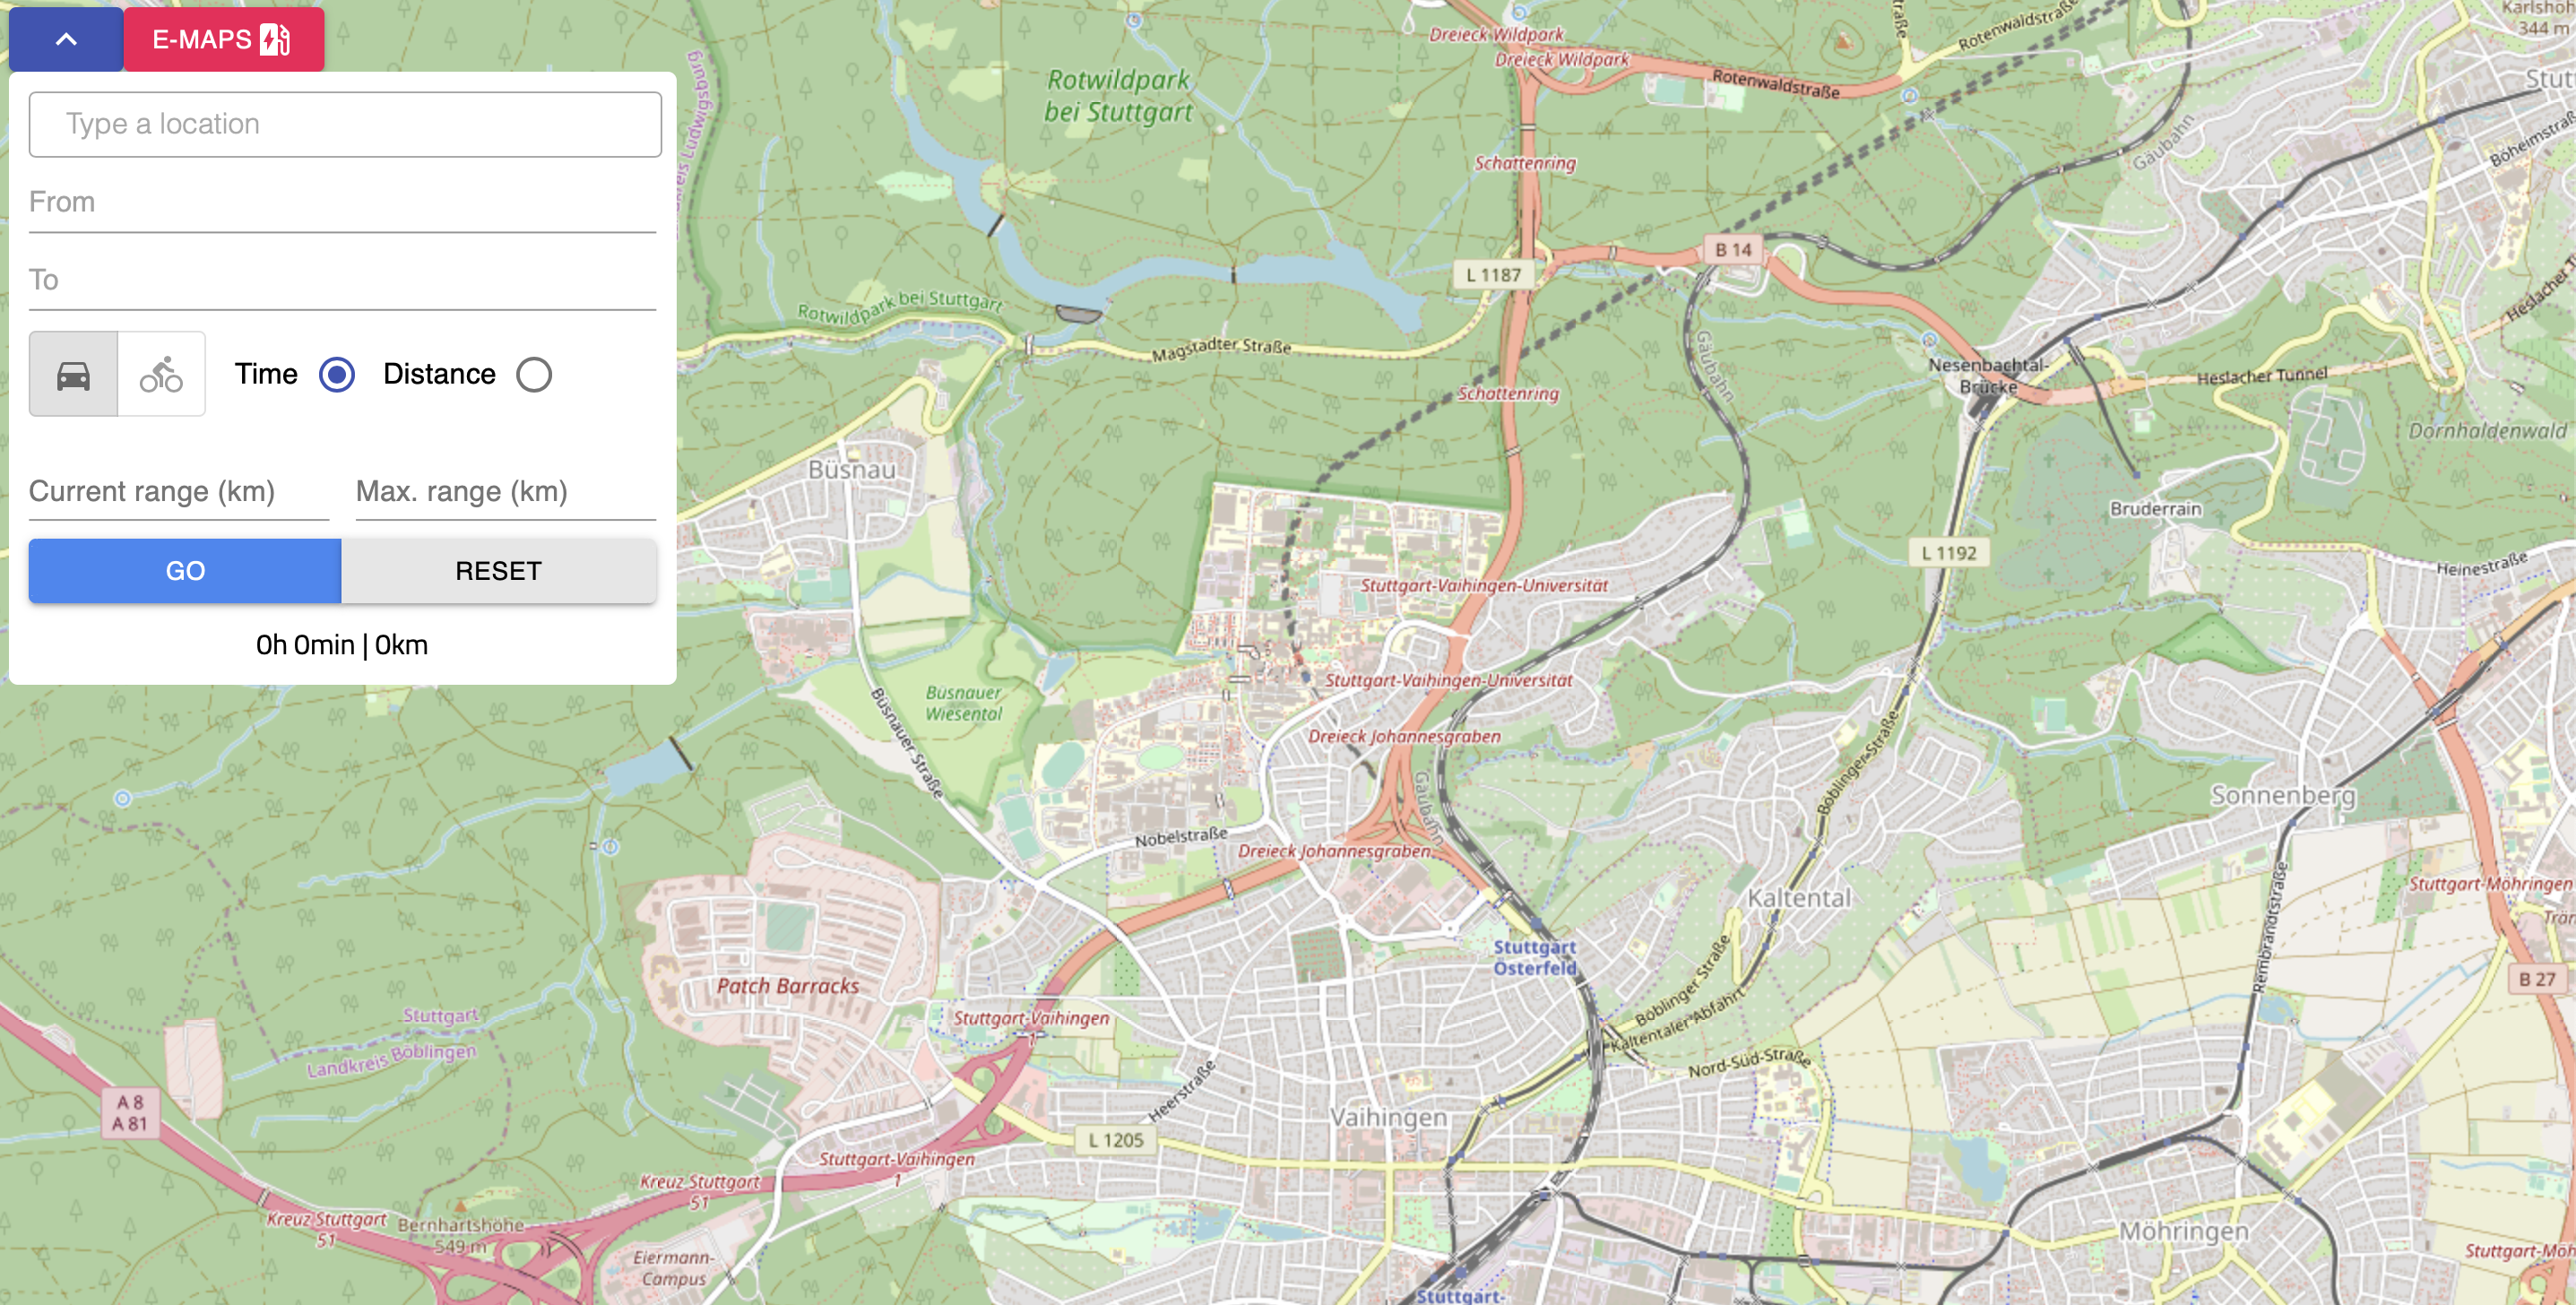
\includegraphics[scale=0.3]{figures/base_ui}
    \caption{Screenshot of the Frontend}
    \label{fig:base_ui}
\end{figure}
\subsection{Features}
\section{Conclusion and Future Work}
\bibliographystyle{alpha}
\bibliography{ref}
\end{document}